\documentclass[main.tex]{subfiles}
\begin{document}
\begin{titlingpage}
\begin{center}

~ \\[3cm]

%\includegraphics[width=0.6\textwidth]{figurer/ASE}~\\[1cm]

\textsc{\LARGE Bilag 2}\\[1.5cm]

%\textsc{\Large Sundhedsteknologi}\\
%\textsc{\Large 3. semesterprojekt}\\[0.5cm]

\noindent\makebox[\linewidth]{\rule{\textwidth}{0.4pt}}\\
[0.5cm]{\Huge Om Dysfagi}
\noindent\makebox[\linewidth]{\rule{\textwidth}{0.4pt}}
\end{center}
\vfill
\begin{center}
{\large 16. december 2017}
\end{center}
\end{titlingpage}

\newpage
\tableofcontents*
\newpage


\chapter{Om Dysfagi}
\section{Indledning}
Når indtagelse af mad og drikke finder sted, passerer det mundhulen, forbi svælget og ned i spiserøret. Denne synkesprocess foregår ved, at bolus skubbes bagud mod svælget ved hjælp af tungen, som presser op og bagud. Derefter udløses en refleks pga. sanseceller i svælget. Dette foregår uden for viljens kontrol og i sammenspil med den forlængede rygmarv. Hele synkeprocessen er et samspil mellem 20-30 muskler, som enten skal trække sig sammen eller slappe af i den rigtige rækkefølge \cite{Sand2008MennesketsFysiologi}. 

Synkeprocessen består af fire sammenhængende faser:
\begin{enumerate}
\item Præ-Oral fase:\\
Denne fase indtræder forud for drikke- og fødindtagelse i munden. Den er karakteriset ved at spytproduktion og synkestimulation starter, når man ser og dufter til mad og drikke \cite [s. 12]{Kjaersgaard2013DifficultiesPerspective}.    
\item Oral fase (i munden): \\
I denne fase bliver maden bidt i stykker i munden. Her tygges maden, som bliver blandet med spyt og formet til en bolle (bolus). Ved hjælp af tungen transporteres bolus til den bagerste del af mundhulen samtidig med at ganespejlet lukker af op til næsen.
\item Faryngeale fase (i svælget): \\ Her bliver bolus transporteret gennem svælget og luftrøret beskyttes ved at stemmebånde og strubelåget lukker, samtidig med at indgangen til spiserøret åbnes.     
\item Esophageal fase (i spiserøret):
Spiserøret indsnævres og bolus transporets til mavesækken vha. en peristaltisk bevægelse \cite [s. 395]{Sand2008MennesketsFysiologi}.
\end{enumerate}

\begin{figure}[H]
\centering
{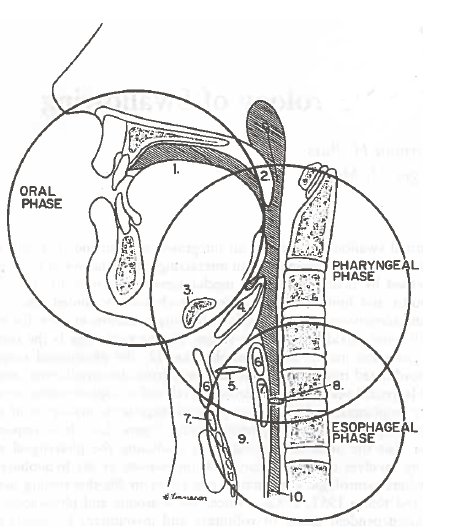
\includegraphics[width=6cm]
{Figure/dysfagi3faser}}
\caption{De tre sidste faser ved synkeprocessen\cite{Bass1992Dysphagia:Management}}
\label{trefaser}
\end{figure}


\section{Hvad er dysfagi?}
Dysfagi er den medicinske betegnelse for symptom relateret til dysfunktion af synkeprocessen \cite{KjaersgaardPh.d.studerendeDYSFAGIKonsekvenser}. Dysfagi tilstanden er karakteriseret ved spise- og drikkevanskeligheder hos patienten. Resultatet kan være en fejlsynkning ved, at bolus ender i luftrøret i stedet for spiserøret. Dette kan bl.a. medføre udvikling af pneumoni.
\section{Hvem får dysfagi?}

 Dysfagi symptomerne kan bl.a. observeres hos patienter med sklerose, apopleksi og parkinson.   Symptomerne forekommer også ved kræft, KOL og almen svækkelse og aldring \cite{SallyRefsgaardTinesterbyKristensen2015DysfagiKommune}. 

Ifølge patientombuddets temarapport fra 2012 om dysfagi at:

\begin{itemize}
\item 60-87 \% af beboere på plejehjem for ældre har synkebesværligheder.
\item 30 \% alle apopleksipatienter har dysfagi. 15.000 danskere rammes hvert år af apopleksi. Forekomsten af dysfagi er ca. 37-78 \% ved akut apopleksi. Hos patienter med i den akutte fase, er dysfagi/aspiration en betydende dødsårsag. Herudover lever 30-40.000 danskere med senfølger efter en apopleksi, nogle har dysfagi
\item 20-50 \% af patienter med Parkinson og Alzheimer har dysfagi. Der lever ca. 6. 000 patienter med Parkinson i Danamark og ca. 45.000 patienter med Alzheimer.  
\item 30-60 \% af patienter med muskelsvind har dysfagi.
\item Herudover er der ca. 10.000 børn, unge og voksne med Cerebral Parese (CP) også kendt som "spastisk lammelse", der har synkebesvær \cite{Bommersholdt2012TemarapportDysfagi}. 
\end{itemize}

\section{Konsekvenser}
Dysfagi kan have følgende konsekvenser \cite[s. 12]{KjaersgaardPh.d.studerendeDYSFAGIKonsekvenser}:
\begin{itemize}
\item Manglende oral ernæring og dermed under- eller fejlernæring
\item Dehydrering
\item Aspiration
\item Kvælning
\item Udvikling af aspirationspneumoni
\item Social isolering
\item Øget risiko for mortalitet
\item Reduceret livskvalitet

\end{itemize}



\section{Nuværende håndtering af dysfagi}


Diagnosticering af øvre dysfagi kan inddeles i en tre-delt model. Den første intervention handler om at screene patientens mentale tilstand ved at vurdere patientens bevidsthedsniveau, orienteringsevne, handlekraft, samt evnen til at synke få konsistenstyper som vand og spytflåd. Hvis det vurderes af klinikeren, at der er behov for yderligere udredning, sendes patienten videre til en klinisk undersøgelse. Den kliniske undersøgelse er baseret på Facial-Oral-Tract-Therapy (F.O.T.T) metoden og anvendes til at vurdere parametre som patientens sensoriske og motoriske respons, åndedræt og oral indtagelse af fødebolus \cite[s. 23-25]{Kjaersgaard2013DifficultiesPerspective}. 

Den kliniske undersøgelse er subjektiv, da det foretages af en klinikker uden hjælp af teknologiske apparater. Denne undersøgelsesmetode mangler præcision til f.eks. at opdage silent aspiration, som kan medføre udvikling af pneumoni og i værste fald kvælning. Derfor anbefales det af sundhedsstyrelsens nationale kliniske retningslinjer for øvre dysfagi, at man supplere den kliniske undersøgelse med en instrumentel undersøgelse til voksne med synkebesvær \cite{Sundhedsstyrelsen2015NationalDysfagi}.

Den instrumentelle undersøgelse omfatter Fiber Endoskopisk Evaluering af Synkefunktionen (FEES) og/eller Funktionel Videoradiologisk Evaluering af Synkefunktionen (FVES).  Ved FEES undersøgelse, som er en invasiv intervention, fører klinikeren en fiberoptisk endoskop gennem patientens næse og pharynx for at få et visuelt billede af pharynx' anatomi. Anormaliteter, som observeres undervejs dokumenteres i en modificeret udgave af ”Der Berliner Dysphagia Index”, som er en standard protokol til dokumentation af FEES undersøgelse \cite{afLambertsenKMDKock-JensenCMDKjrsgaardAMScOTHansenTSMsci/MPHWestergaardLMD2007ModificeretIndex}. 

Undersøgelsen kan afdække patientens synkevanskeligheder ved at iagttage aspiration af bolus i luftvejene, tilstedeværelsen af bolus-rester i strubehovedet og patientens evne til at synke egen saliva \cite[s. 27-28]{Kjaersgaard2013DifficultiesPerspective}. 
Ved FVES undersøgelse anvendes røntgenstråler, som muliggør visualisering af fødebolus i alle faser. Klinikeren kan vha. denne metode evaluere om pharyngeal eller øsophageal muskler fungerer korrekt og om patienten kan kompensere for dysfagien med reflektoriske teknikker som fx ændring af hovedstilling. FEES og FVES anvendes som ”guld standarder” ved diagnosticering af patienter med øvre dysfagi, og begge undersøgelsesmetoder betragtes som komplementære værktøjer til udredning af dysfagi frem for konkurrerende \cite[s. 50]{Kjaersgaard2013DifficultiesPerspective}.



\bibliography{Mendeley.bib}
\end{document}